% LaTeX template for DLD Lab - runs with MikTeX and other platforms

\documentclass{article}
\usepackage{mathptmx}
\usepackage{amssymb}
\usepackage{amsfonts}
\usepackage{amsmath}
\usepackage{latexsym}
\usepackage{setspace}
\usepackage{verbatim}

\usepackage[dvipsnames]{xcolor}
\usepackage{matlab-prettifier}
\usepackage{float}
\usepackage[export]{adjustbox}



\numberwithin{equation}{section}
\newtheorem{thm}{Theorem}[section]
\newtheorem{dfn}[thm]{Definition}
\newtheorem{lem}[thm]{Lemma}
\newtheorem{rem}[thm]{Remark}
\newtheorem{cor}[thm]{Corollary}
\newtheorem{prop}[thm]{Proposition}
\newtheorem{asm}[thm]{Assumption}
\newtheorem{example}[thm]{Example}

\newenvironment{proof}{\noindent {\bf Proof.\/}}{$\qed$\vskip 0.1in}
\def\qed{ \hfill \vrule width.2cm height.2cm depth0cm\smallskip}

\usepackage{xcolor}
\usepackage{listings}
\usepackage{pythonhighlight}

\definecolor{mGreen}{rgb}{0,0.6,0}
\definecolor{mGray}{rgb}{0.5,0.5,0.5}
\definecolor{mPurple}{rgb}{0.58,0,0.82}
\definecolor{backgroundColour}{rgb}{0.95,0.95,0.92}

\lstdefinestyle{CStyle}{
    backgroundcolor=\color{backgroundColour},   
    commentstyle=\color{mGreen},
    keywordstyle=\color{magenta},
    numberstyle=\tiny\color{mGray},
    stringstyle=\color{mPurple},
    basicstyle=\footnotesize,
    breakatwhitespace=false,         
    breaklines=true,                 
    captionpos=b,                    
    keepspaces=true,                 
    numbers=left,                    
    numbersep=5pt,                  
    showspaces=false,                
    showstringspaces=false,
    showtabs=false,                  
    tabsize=2,
    language=C
}

\DeclareMathOperator*{\argmax}{argmax} % thin space, limits underneath in displays


% For minted -> Python
\usepackage{tcolorbox}
\tcbuselibrary{minted,breakable,xparse,skins}
\definecolor{bg}{gray}{0.95}
\DeclareTCBListing{mintedbox}{O{}m!O{}}{%
  breakable=true,
  listing engine=minted,
  listing only,
  minted language=#2,
  minted style=default,
  minted options={%
    linenos,
    gobble=0,
    breaklines=true,
    breakafter=,,
    fontsize=\small,
    numbersep=8pt,
    #1},
  boxsep=0pt,
  left skip=0pt,
  right skip=0pt,
  left=25pt,
  right=0pt,
  top=3pt,
  bottom=3pt,
  arc=5pt,
  leftrule=0pt,
  rightrule=0pt,
  bottomrule=2pt,
  toprule=2pt,
  colback=bg,
  colframe=orange!70,
  enhanced,
  overlay={%
    \begin{tcbclipinterior}
    \fill[orange!20!white] (frame.south west) rectangle ([xshift=20pt]frame.north west);
    \end{tcbclipinterior}},
  #3}



\numberwithin{equation}{section}
\newcommand{\cA}{\mathcal{A}}
\newcommand{\cB}{\mathcal{B}}
\newcommand{\cC}{\mathcal{C}}
\newcommand{\cD}{\mathcal{D}}
\newcommand{\cE}{\mathcal{E}}
\newcommand{\cF}{\mathcal{F}}
\newcommand{\cG}{\mathcal{G}}
\newcommand{\cH}{\mathcal{H}}
\newcommand{\cI}{\mathcal{I}}
\newcommand{\cJ}{\mathcal{J}}
\newcommand{\cK}{\mathcal{K}}
\newcommand{\cL}{\mathcal{L}}
\newcommand{\cM}{\mathcal{M}}
\newcommand{\cN}{\mathcal{N}}
\newcommand{\cO}{\mathcal{O}}
\newcommand{\cP}{\mathcal{P}}
\newcommand{\cQ}{\mathcal{Q}}
\newcommand{\cR}{\mathcal{R}}
\newcommand{\cS}{\mathcal{S}}
\newcommand{\cT}{\mathcal{T}}
\newcommand{\cU}{\mathcal{U}}
\newcommand{\cV}{\mathcal{V}}
\newcommand{\cW}{\mathcal{W}}
\newcommand{\cX}{\mathcal{X}}
\newcommand{\cY}{\mathcal{Y}}
\newcommand{\cZ}{\mathcal{Z}}
%greeks
\newcommand{\te}{{\theta}}
\newcommand{\Te}{{\Theta}}
\newcommand{\vt}{{\vartheta}}
\newcommand{\Om}{{\Omega}}
\newcommand{\om}{{\omega}}
\newcommand{\ups}{{\upsilon}}
\newcommand{\ve}{{\varepsilon}}
\newcommand{\del}{{\delta}}
\newcommand{\Del}{{\Delta}}
\newcommand{\gam}{{\gamma}}
\newcommand{\Gam}{{\Gamma}}
\newcommand{\vf}{{\varphi}}
\newcommand{\Sig}{{\Sigma}}
\newcommand{\sig}{{\sigma}}
\newcommand{\al}{{\alpha}}
\newcommand{\be}{{\beta}}
\newcommand{\ka}{{\kappa}}
\newcommand{\la}{{\lambda}}
\newcommand{\La}{{\Lambda}}


\def \D{\mathbb{D}}
\def \E{\mathbb{E}}
\def \F{\mathbb{F}}
\def \H{\mathbb{H}}
\def \L{\mathbb{L}}
\def \M{\mathbb{M}}
\def \N{\mathbb{N}}
\def \P{\mathbb{P}}
\def \Q{\mathbb{Q}}
\def \R{\mathbb{R}}
\def \Z{\mathbb{Z}}
\def \Sb{\mathbb {S}}

\def \om{\omega}
\def \Om{\Omega}
\def \ep{\epsilon}

\def\reff#1{{\rm(\ref{#1})}}

\usepackage{times}	   % uncomment to use Times-Roman fonts
%\usepackage{mathpazo}     % uncomment to use Palatino fonts
\usepackage{amsmath}	   % enable amsmath features
\usepackage{graphicx}      % enable inclusion of eps graphs
\usepackage{cite}          % bibliographical citations
\usepackage{url}           % typesetting URL's
\usepackage{color}

% ---------------------------------------------------------------

\setlength{\textwidth}{5.75in}            
\setlength{\oddsidemargin}{0.375in}   % textwidth + 2*oddsidemargin = 6.5
\setlength{\evensidemargin}{0.375in}
\setlength{\topmargin}{-0.5in}
\setlength{\textheight}{9in}

\def\ce{\begin{center}}            
\def\cend{\end{center}}

\def\red{\color{red}}
\def\blue{\color{blue}}
\def\black{\color{black}}

\begin{document}

\ce
\red\Large
RUTGERS UNIVERSITY \\[0.05in]
School of Engineering \\[0.05in]
Department of Electrical \& Computer Engineering \\[0.2in]
\blue ECE 472 -- Robotics \& Computer Vision-- Fall 2022
\cend

\vspace{1in}

\huge \blue 

\begin{center}
Project 2 - Reinforcement Learning: Cart Pole
\end{center}

\vspace{1in}

\Large

Name (last, first) : \ Mehmet Ali Soner 

\vspace{0.3in}

netID : \ mas996

\vspace{0.3in}

RUID:  196000499

\vspace{0.3in}

Date: \today




\vspace{1in}

\color{black} \normalsize


\newpage




\section*{Problem 1}
For this section, I have followed the CartPole tutorial from pytorch's official website. I am going through the details of that specific tutorial in this section. However, the performance of this model turned out to be unstable and poor. In order to get better performance and video results, I switched over to the github commit that was provided one of our fellow students. The results you see in the Jupyter Notebook and the performance metric plots are obtained through the \textbf{github commit} code. The specific link for that github repo is: \url{https://github.com/SiftingSands/tutorials/blob/DQN_revise_training/intermediate_source/reinforcement_q_learning.py}. Now, the detailed of the pytorch tutorial:

\begin{mintedbox}{python}
!apt-get update
!apt-get install -y xvfb x11-utils
%pip install pyvirtualdisplay==0.2.*
%pip install gym[classic_control]
\end{mintedbox}

I am calling apt-get update since I ran into issues with xvfb couple of times and this seem to resolve it. We install xvfb and pyvirtualdisplay for the video capturing. Then we import the gym package and create the environment for "CartPole":

\begin{mintedbox}{python}
import gym
if gym.__version__ < '0.26':
    env = gym.make('CartPole-v0', new_step_api=True, render_mode='single_rgb_array').unwrapped
else:
    env = gym.make('CartPole-v0', render_mode='rgb_array').unwrapped
\end{mintedbox}

After this, I will skip few things such as the video capturing and importing other various packages. I want to focus on the DQN's linear layer. In this model, we have to have two possible outputs in our final/linear layer since we will either push the cart to the right or to the left. In order to add this layer, we have to know the output size of each convolutional layer so that we have the right input size for the linear layer. That's why we call conv2d\_size\_out three times since we have three convolutional layers. We then calculate the input size and add it with: 

\begin{mintedbox}{python}
class DQN(nn.Module):
# Architecture code (3 conv layers, 3 batch norms)
...
        def conv2d_size_out(size, kernel_size = 5, stride = 2):
            return (size - (kernel_size - 1) - 1) // stride  + 1
        convw = conv2d_size_out(conv2d_size_out(conv2d_size_out(w)))
        convh = conv2d_size_out(conv2d_size_out(conv2d_size_out(h)))
        linear_input_size = convw * convh * 32
        self.head = nn.Linear(linear_input_size, outputs)
\end{mintedbox}

We then implement two functions that will get the cart's location on the screen and will get the screend itself:

\begin{mintedbox}{python}
def get_cart_location(screen_width):
world_width = env.x_threshold * 2
    scale = screen_width / world_width
    return int(env.state[0] * scale + screen_width / 2.0)  # MIDDLE OF CART

def get_screen():
screen = env.render().transpose((2, 0, 1))
    # Cart is in the lower half, so strip off the top and bottom of the screen
    _, screen_height, screen_width = screen.shape
...
cart_location = get_cart_location(screen_width)
...
screen = screen[:, :, slice_range]
\end{mintedbox}

I have mainly included the important lines of the two functions in the snippet. These two functions are crucial since we can describe the current state of the agent through the location of the cart on the screen. We achieve this with some algebra and the information we have about the environment's/simulation's dimensions. \\

Now we get to the part where we train the DQN.
First we initialize the network, the optimization function and the memory.

\begin{mintedbox}{python}
n_actions = env.action_space.n
policy_net = DQN(screen_height, screen_width, n_actions).to(device)
target_net = DQN(screen_height, screen_width, n_actions).to(device)
target_net.load_state_dict(policy_net.state_dict())
target_net.eval()

optimizer = optim.RMSprop(policy_net.parameters())
memory = ReplayMemory(10000)
\end{mintedbox}

$n\_actions$ is the amount of actions we can take in the environment. In this case, it will be two (move cart to right or left). Then, we initialize the policy and the target network. This is mainly for stability since it servers as a "back-up" of the policy network. The target network is basically a copy of the policy network with frozen parameters that get updated once in a while (we copy the parameters into target\_net on line 5 and put the network in eval mode on line 6). So, if overfitting or other errors were to happen in the policy network, the target network is there for stability. On line 6, we initialize the memory by creating a ReplayMemory object. The ReplayMemory class looks like this:

\begin{mintedbox}{python}
Transition = namedtuple('Transition',
                        ('state', 'action', 'next_state', 'reward'))
class ReplayMemory(object):

    def __init__(self, capacity):
        self.memory = deque([],maxlen=capacity)

    def push(self, *args):
        """Save a transition"""
        self.memory.append(Transition(*args))

    def sample(self, batch_size):
        return random.sample(self.memory, batch_size)

    def __len__(self):
        return len(self.memory)
\end{mintedbox}

The ReplayMemory class can hold Transition and  can return random Transitions of a certain batch size. This is crucial since the policy network will learn from recent Transition tuples in the ReplayMemory object. It will use that information to optimize the model, to achieve a better policy. So, the memory object serves as the memory for the training.\\

Next, I will explain some details in the select\_action() and optimize\_model() function. The way we choose an action is the following:

\begin{mintedbox}{python}
def select_action(state):
...
    sample = random.random()
    eps_threshold = EPS_END + (EPS_START - EPS_END) * \
        math.exp(-1. * steps_done / EPS_DECAY)
    steps_done += 1
    if sample > eps_threshold:
        with torch.no_grad():
            return policy_net(state).max(1)[1].view(1, 1)
    else:
        return torch.tensor([[random.randrange(n_actions)]], device=device, dtype=torch.long)
\end{mintedbox}
Given an input state, we select the action. First, we get a random value and compare it to our epsilon threshold. If this random value is over the threshold, we go through the policy net with the input state and take the action with the highest reward. If the random value doesn't cross the threshold, we then select a random action out of the possible actions in this environment (right, left). With this function, we can now define the model optimization function. \\

The optimize\_model() function is where the RL algorithm is implemented. First, I will explain how we "load" the necessary data.

\begin{mintedbox}{python}
def optimize_model():
    if len(memory) < BATCH_SIZE:
        return
    transitions = memory.sample(BATCH_SIZE)
    batch = Transition(*zip(*transitions))
\end{mintedbox}

We first try to get a batch of Transitions into the model. If there isn't enough Transitions in the memory, we return. If we have enough information stored in the memory, we load a sample from there. Then, we create a batch variable from the transitions variable. The batch holds all the information regarding the state, action, reward and next state. Then, we divide each information from the batch into individual variables.

\begin{mintedbox}{python}
non_final_mask = torch.tensor(tuple(map(lambda s: s is not None,
                                          batch.next_state)), device=device, dtype=torch.bool)
    non_final_next_states = torch.cat([s for s in batch.next_state
                                                if s is not None])
    state_batch = torch.cat(batch.state)
    action_batch = torch.cat(batch.action)
    reward_batch = torch.cat(batch.reward)
\end{mintedbox} 

On line 1, we are extracting every next state that is not final, which is not None and storing them as a boolean. True for every non-final state and False for final states. This will be helpful afterwards when we will compute the values of the next states. On line 3, we do same thing, except we store the values of the states. Line 5-7, we extract information about states, rewards and actions from the batch and store them into individual variables. Afterwards, we compute the state action values like this:

\begin{mintedbox}{python}
state_action_values = policy_net(state_batch).gather(1, action_batch)
\end{mintedbox}

We pass through the policy net with the state batch as the input and observe, which action the policy net would have taken. We get these from our action\_batch variable. Next step is to calculate the next state values:

\begin{mintedbox}{python}
next_state_values = torch.zeros(BATCH_SIZE, device=device)
next_state_values[non_final_mask] = target_net(non_final_next_states).max(1)[0].detach()
\end{mintedbox}

On line 1, we allocate space for the results for our computation we are going to perform on line 2. On line 2, we pass through the target net with obtained next\_state\_values variable and extract the result/action that has the highest reward with the max function. We are using the target net for the improved stability that we mentioned before. The target net that is called on this line is the "old" target net that is constant. Another detail worth explaining is the significance of the non\_final\_mask variable. This is needed here since we will store a value in to next\_state\_values if the state was non-final and 0 if the state was final. This is determined by the values in the non\_final\_mask variable. The last important line of code in this function is the following:
\begin{mintedbox}{python}
expected_state_action_values = (next_state_values * GAMMA) + reward_batch
\end{mintedbox} 
This is where we actually compute which action to take in order to get to the next state for each state. We multiply the next\_state\_values by gamma in order to guarantee convergence and add the rewards to it. This equation can be found under the DQN algorithm page in the tutorial, where the policy function is described. \\

For the training loop, the main structure looks like this:

\begin{mintedbox}{python}
num_episodes = any_number
for i_episode in range(num_episodes):
    # Initialize the environment and state
    env.reset()
    last_screen = get_screen()
    current_screen = get_screen()
    state = current_screen - last_screen
	...
	for t in count():
        # Select and perform an action
        action = select_action(state)
        _, reward, done, _, _ = env.step(action.item())
        reward = torch.tensor([reward], device=device)

        # Observe new state
        last_screen = current_screen
        current_screen = get_screen()
        if not done:
            next_state = current_screen - last_screen
        else:
            next_state = None

        # Store the transition in memory
        memory.push(state, action, next_state, reward)

        # Move to the next state
        state = next_state

        # Perform one step of the optimization (on the policy network)
        optimize_model()
        if done:
            break

        # Update the target network, copying all weights and biases in DQN
        if t % TARGET_UPDATE == 0:
            target_net.load_state_dict(policy_net.state_dict())
\end{mintedbox}

We iterate through the model for num\_episodes times. In each episode, we first reset the environment, initialize the screen, get the current and the last screen, which are identical at the start. The main reason why we reset the environment is because episodes are finished after a certain time period or they fail. So, we have to start again. Then on line 9, we start the episode. We call the select\_action() that will return an action that we will input into the environment on line 12. This line of code steps through the environment and applies the inputted action in the environment. As the output, we get the reward and a boolean that indicates if this was a final state. We update the states by storing the current\_screen into last\_screen. This can be applied since we simulated the action in the environment on line 12, thus changed the actual current state. The current\_screen variable holds the old screen after this. In order to update current\_screen, we just call get\_screen(). Based on the done variable, we either restart or we calculate the next\_state, which is the difference between the current and the last screen, and transition into that. Before going to the next iteration in the loop, we save the necessary data from this transition and call optimize\_model(). Every now and then we also update the target net's parameters as seen on line 35-36.



\section*{Problem 2}
In reinforcement learning, we want to create a policy function $\pi$ that will maximize the reward in a given state $s$ after performing some action $a$ in a certain environment. The function that computes the reward from $s$ and $a$ is the $Q$ function. In the CartPole case,
\begin{itemize}
\item the states: 
\begin{itemize}
\item the cart's x-coordinate
\item cart's velocity
\item the pole's angular velocity
\item the pole's angle
\end{itemize}
\item the environment: the simulation that is simulating cart with the pole that is on a rail
\item actions:
\begin{itemize}
\item move cart to right
\item move cart to left
\end{itemize} 
\item reward:
\begin{itemize}
\item reward = 1, when the pole stays within the specified angle (±12°) and cart's x-coordinate is in range of (-2.4, 2.4)
\item reward = 0, when the above mentioned conditions are not met, then we fail and restart the environment
\end{itemize} 
\end{itemize}  

Essentially we want:
$$
\pi^*(s) = \argmax_a \ Q^*(s,a)
$$
However, we cannot achieve this since we don't know every possible state, action and reward in the world. What we do instead is, we try to approximate the $Q$ function with the help of neural networks. We assume that the $Q$ function is a Bellman equation and can write it like this:

$$
Q^{\pi}(s,a) = r_0 + \gamma Q^{\pi}(s',\pi(s'))
$$
This equation describes that the current $Q$ function is the sum of the current reward $r_0$ and the $Q$ function of the future state $s'$ and action $a' = \pi(s')$ multiplied by a discount rate $\gamma$. This is a very powerful tool since we can describe the $Q$ function recursively.

We can rewrite this equation into what will be inputted into the Huber loss.
For the Huber loss function, we input what is called the temporal difference error, $\delta$:
$$
\delta = Q(s,a) - \left(r_0 + \gamma \max_a Q(s',\pi(s'))\right)
$$
The first term of the subtraction is the prediction, the values that we get when we take an action $a$ in the state $s$. We get this value when we are inputting the state\_batch into the policy\_net to get the state\_action\_values. The second term of the subtraction is the target value that we obtain by passing through the target\_net with non\_final\_next\_states. The results of that pass through are the next\_state\_values. We then multiply the next\_state\_values by $\gamma$ and add the reward batch to it. $s'$ would be the future state, $a'$ the future action.  We want to minimize this error since we want to have our prediction and target values as close as possible to each other. We do that by inputting that into a Huber loss function. 










\section*{Problem 3}
For performance metrics, we can observe the duration of each episode or the reward. This gives us basic understanding of how well the model performs. For every action where the pole is still upright, we add +1 to the reward variable we have or we add up every action that didn't result into a final state and include the terminating state as well. We do this with a for loop and the iteration variable in the loop condition:


\begin{mintedbox}{python}
for t in count():
	if isRandom  == True:
	  action = torch.tensor([[env.action_space.sample()]], device=device, dtype=torch.long)
	else:
	  action = select_action(state,policy_net)
	observation, reward, terminated, truncated, _ = env.step(action.item())
	reward = torch.tensor([reward], device=device)
	done = terminated or truncated

	...
	
	if done:
		episode_durations.append(t + 1)
		break
\end{mintedbox}

This is how the loop for each episode looks like. When we have a terminal state, then we go into the if statement on line 12 and add how many steps we have taken, which equals to the duration of one episode. We then plot these duration with a helper plotting function. Here are the result of three scenarios, namely:
\begin{enumerate}
\item A random agent with num\_episodes = 600
\item A trained agent with num\_episodes = 100
\item A trained agent with num\_episodes = 600
\end{enumerate}


Here are the results in that order:

\begin{figure}[H]
	\centering
	
	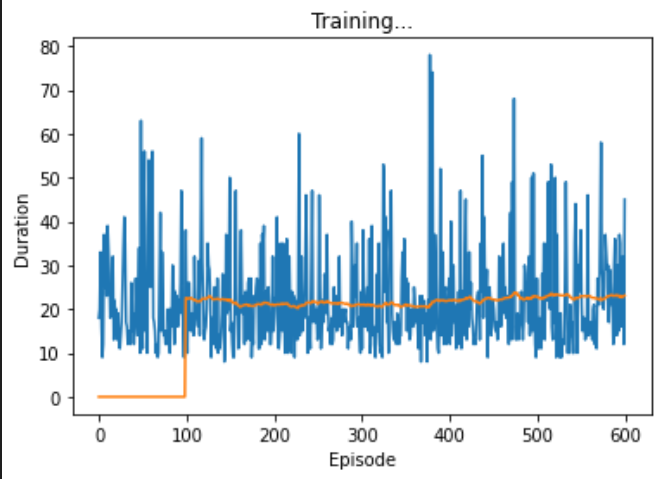
\includegraphics[width=\linewidth,cframe=blue 2.5pt 2.5pt]{random_agent.png}
	\\	
	\vspace{0.1in}
	\textbf{Fig.1:} A random agent with num\_episodes = 600
	\\
	\label{fig:Fig.1}
\end{figure}



\begin{figure}[H]
	\centering
	
	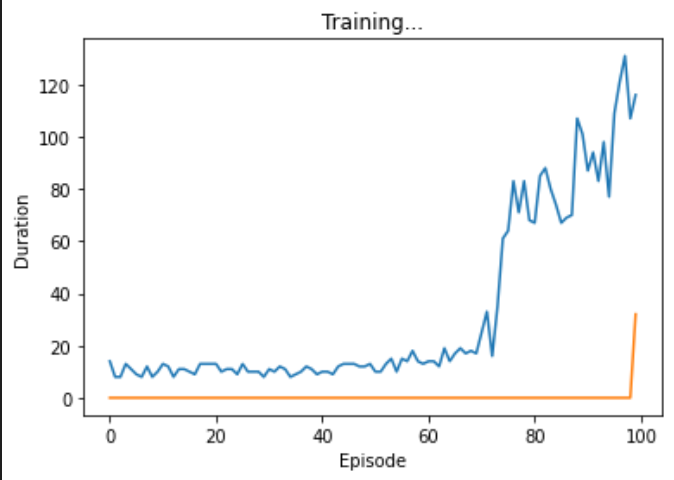
\includegraphics[width=\linewidth,cframe=blue 2.5pt 2.5pt]{agent100.png}
	\\	
	\vspace{0.1in}
	\textbf{Fig.2:} A trained agent with num\_episodes = 100
	\\
	\label{fig:Fig.2}
\end{figure}

\begin{figure}[H]
	\centering
	
	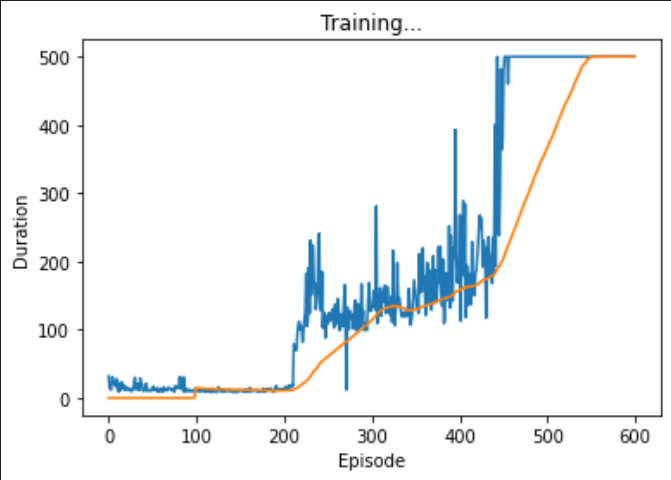
\includegraphics[width=\linewidth,cframe=blue 2.5pt 2.5pt]{agent600.png}
	\\	
	\vspace{0.1in}
	\textbf{Fig.3:} A trained agent with num\_episodes = 600
	\\
	\label{fig:Fig.3}
\end{figure}


The results are as expected. The worst performance out of the three is with the random agent, the second worst is the agent with the small training time (or less number of episodes) and the best performance comes from the trained agent with the highest training time. In Fig.1, we can observe that the episode duration on average stays constant and has a value of 25-30. This makes sense since the agent doesn't update it's policy net efficiently because it is selecting random action. There are some outliers that happen (peak at 79 and 70) because of the randomness of the action selection module. The module might take the all of the right actions in one episode. However, the probability of that happening is low because it has to randomly select all of the actions successively and it is reflected in this plot. 

The second figure, Fig.2, shows more promising results. The performance in the first 70 episodes is in fact worse the the first 70 episodes with a random agent but there is sharp jump in performance around episode 80. Here, we can see that the performance significantly increases and stays at this level. We can also conclude that training an agent for 100 episodes isn't quite enough since it doesn't pass the "solved" threshold of 200 in this environment. The results seem promising however and we can predict that the duration of each episode is going to increase with more training. This agent outperforms the random agent even though it had 1/6 of episodes to train in.

The third figure, Fig.3, proves our prediction we had with Fig.2. Again, around 100 episodes there is a sharp peak that seems to be constant until episode = 200. From there, there is a linear increase in performance until episode = 450 from where the performance increase improves even further. The performance increase is a lot steeper. It is also around episode = 450, where the module passes the "solved" threshold of 200. After some time, the module cannot improve any further and it stagnates at around episode = 550. This is all expected and seems ordinary. What is surprising is that both train models had much worse performance in the first 60-80 episodes than the random agent. The performance in the first hundred episode also seem to decrease when we increase the number of episodes we want the model to simulate. This doesn't matter since we can arrive a higher episode duration or overall reward in the long run.


\section*{Problem 4}
Here are three other problems that can be solved with RL on open-AI gym:

\begin{enumerate}
\item Mountain Car (Classic Control):
\begin{itemize}
\item State: In this environment, there are only two states. The position of the car along the x-axis and the velocity of the car. The x-coordinate and the velocity of the car can from $\left(-\infty, \infty\right)$.
\item Action: There are three actions in this environment. Accelerate to the right, accelerate to the left or don't accelerate at all.  
\item Environment: A car is at the bottom of a "sinusoidal valley" and has to get out of that valley by reaching the flag at the top of the hill. The starting position of the car is a random value in the range of [-0.6,-0.4]. The episode ends when the car's x-coordinate is greater than or equal to 0.5, which means it has reached the flag or when the episode length is over 200.
\item Reward: In this environment, the reward is -1 for each timestep where the car hasn't reached the flag on top of the hill. So, the car has to reach the flag as quickly as possible.  
\end{itemize}



\item Car Racing (Box2D): 
\begin{itemize}
\item State: In this environment, the observation space consists of 96x96 pixels, which determine the track and the position of the racing car.
\item Action: There are three actions if the environment is continuous and 5 if discrete. In the continuous scenario we have: steering (-1 full left, +1 full right), gas and break. In the discrete scenario, we have: do nothing, turn right, turn left, gas, brake.
\item Environment: A racing car is on a racing track and is trying to complete it. It starts at the starting point of the track, in the middle of center of the road. The episode ends when all tiles have been visited. The racing car can go off the track but it will get rewarded with -100 and "die" per the Gym documentation.
\item Reward: In this environment, the reward is -0.1 for every frame that the car took to get to the episode's end and +1000/N, where N is the amount of tiles that the car visited.
\end{itemize}









\item : Frozen Lake (Toy Text):
\begin{itemize}
\item State: In this environment, the observation space consists of one numeric value, which indicates the position of the agent on the lake. It can be calculated with $agent{position} = current\_row * nrows + current\_col$.
\item Action: There are four actions that the agent can take in this environment. Go up, left, down and right.
\item Environment: An agent has to reach a goal $G$ on a frozen lake with holes $H$ from the starting point $S$. The main objective is to reach the goal \textbf{without} falling into one of the holes. The agent's movement may not be clear since it will not move into the direction of the goal all the time. This is simply because of the slippery nature of the frozen lake.
\item Reward: In this environment, the only time you get a +1 is when you reach the goal. All other actions resulting into reaching a hole or any frozen tile, "pay out" a 0 as reward.
\end{itemize}


\end{enumerate}





\begin{comment}
\begin{figure}[H]
	\centering
	
	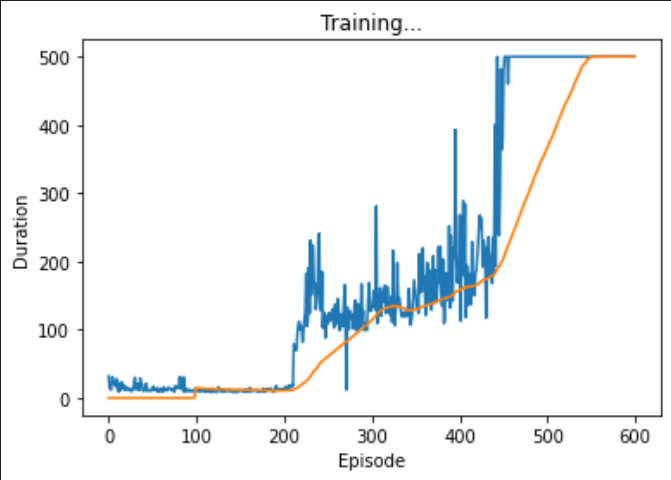
\includegraphics[width=\linewidth,cframe=blue 2.5pt 2.5pt]{agent600.png}
	\\	
	\vspace{0.1in}
	\textbf{Fig.3:} A trained agent with num\_episodes = 600
	\\
	\label{fig:Fig.3}
\end{figure}
\end{comment}













\end{document}